

\section{Введение}
Для определения величины отношения заряда электрона к постоянной
Больцмана в данной лабораторной работе используется метод, основанный на исследовании
процессов, протекающих в биполярном транзисторе.



\subsection{Задачи работы}

Таким образом, задачами данной работы являются:
\begin{enumerate}
    \item Измерить зависимость тока короткого замыкания коллектора биполярного
транзистора от напряжения между эмиттером и базой.
    \item По результатам измерений определить отношение заряда электрона к
постоянной Больцмана.
\end{enumerate}




\section{Основная часть}

\subsection{Теоретическая часть}
\subsubsection{P-n-переход}
P-n-переход представляет собой контактную область между двумя полупроводниковыми материалами с разными типами проводимости: p-типа (преобладает дырочная проводимость) и n-типа (преобладает электронная проводимость).
\parОсновой для создания p-n-перехода служит 4-валентный полупроводник (чаще всего кремний Si, реже германий Ge). Путём легирования (внедрение небольших количеств примесей других металлов) такого материала происходит изменение его электрических свойств:
\begin{itemize}
\itemДонорная примесь (например, As,) – пятивалентные атомы, создающие избыток электронов (n-тип).
\itemАкцепторная примесь (например, B,) – трёхвалентные атомы, образующие дефицит электронов (дырки) (p-тип).
\end{itemize}
\parПри контакте полупроводников p- и n-типа на атомарном уровне формируется p-n-переход. В этой пограничной зоне возникает диффузионный ток: Электроны и дырки хаотично перетекают из той области,
где их больше, в ту область, где их меньше, и рекомбинируют друг с другом.
В результате в области перехода образуется так называемая обеднённая зона, где концентрация подвижных носителей заряда (свободных электронов и дырок) мала.
\parВ приграничной зоне полупроводника p-типа, прилегающей к границе, образуется отрицательный заряд за счет поступления электронов. В то же время в приграничной области полупроводника n-типа возникает положительный заряд из-за потери электронов, что эквивалентно появлению дырок. Это распределение зарядов создает электрическое поле, вызывающее дрейфовый ток, который направлен противоположно диффузионному току. Со временем между этими токами устанавливается равновесие, соответствующее определенной ширине обедненной области.

Ключевой особенностью p-n перехода является односторонняя проводимость, которая лежит в основе принципа действия полупроводникового диода. Добавление внешнего электрического поля нарушает динамическое равновесие в обедненной области.
\begin{itemize}
\itemЕсли внешнее поле направлено противоположно полю p-n перехода, диффузионный ток начинает преобладать над дрейфовым, резко возрастая с увеличением напряжения. При этом обедненная область сужается, переход открыт. Такое подключение называется прямым смещением, а протекающий ток — прямым током.
\itemПри обратном смещении (когда полярность внешнего поля совпадает с полем p-n перехода) внешнее поле усиливает барьер, подавляя диффузионный ток, и основной вклад вносит малый дрейфовый ток. В этом случае переход закрыт.
\end{itemize}
\subsubsection{Устройство и принцип действия биполярного транзистора}
Биполярный транзистор состоит из кристалла полупроводника (типа p или n), в котором сформированы два расположенных рядом p-n перехода. Его можно представить как три чередующихся слоя с разной проводимостью: эмиттер, база и коллектор.

В зависимости от последовательности слоёв различают два типа транзисторов:
\begin{itemize}
\item n-p-n (эмиттер – n-полупроводник, база – p-полупроводник, коллектор – n-полупроводник);
\item p-n-p (эмиттер – p-полупроводник, база – n-полупроводник, коллектор – p-полупроводник).
\end{itemize}
Оба перехода (эмиттер-база и коллектор-база) обладают разными свойствами: эмиттер сильнее легирован, чем база и коллектор, а коллектор имеет большую массу по сравнению с эмиттером. Кроме того, p-n переход между базой и коллектором отличается большими геометрическими размерами.
В цепи э-б p-n в биполярном
транзисторе, включенном по схеме с общей базой в нормальном активном режиме переход смещен в прямом направлении. Электроны из n-области легко переходят в базу (p-типа), где, из-за малой ширины и слабого легирования, большинство не рекомбинирует и достигает коллектора. Там их ускоряет внешнее электрическое поле, создавая коллекторный ток. Дырочная составляющая тока мала из-за низкой концентрации дырок в n-области коллектора. Таким образом, в n-p-n транзисторе ток формируется преимущественно электронами.
\subsubsection{Ток короткого замыкания коллектора биполярного транзистора}
Ток короткого замыкания коллектора $I_{к}$ как функция напряжения
между эмиттером и базой $U_{эб}$ определяется следующим выражением:
\begin{equation}
    I_{\mathrm{k}} = I_{0} \left(e^{\frac{e U_{\text{эб}}}{k T}} - 1\right)
    \label{eq:eq1}
\end{equation}
где $I_{0}$ - ток насыщения, T - температура в К, e - заряд электрона, k - постоянная Больцмана.
\parМожно заметить, что при комнатной температуре и напряжении $U_{эб}$ порядка 0,5-1,0В, показатель степени экспоненты в уравнении (\ref{eq:eq1}) значительно больше единицы. Поэтому приближённо формула принимает такой вид:
\begin{equation}
    I_{\mathrm{k}} = I_{0} \left(e^{\frac{e U_{\text{эб}}}{k T}}\right)
    \label{eq:eq2}
\end{equation}
Для решения уравнения (\ref{eq:eq2}) относительно $\frac{e}{k}$ прологарифмируем его:
\begin{equation}
    \ln I_k = \ln I_0 + \frac{e}{k T} U_{\text{эб}}
    \label{eq:eq3}
\end{equation}
\parВеличины $ln I_k$ и $U_{\text{эб}}$ измеряются в ходе эксперемента. Для решения уравнения (\ref{eq:eq3}) относительно $\frac{e}{k}=T\cdot tg(\alpha)$ необходимо воспользоваться методом парных точек, который позволит определить $tg(\alpha)$.
\begin{equation}
    T\cdot tg(\alpha)=\frac{e}{k}
    \label{eq:eq4}
\end{equation}
\subsection{Эксперимент}
Лабораторная работа заключается в измерении вольтметром напряжения  $U_{\text{кб}}$ в зависимости от задаваемого напряжения $U_{\text{эб}}$.
\parВ лаборатории была зарегистрирована температура $t = {23 \pm 0.5}{^\circ}C$, которая равняется $T = 296{,}15\pm 0{,}5\,\text{К}$.
\parБыло проведено два блока измерений напряжений $U_{\text{кб}}$. В первом случае для измерения задаваемого напряжения $U_{\text{эб}}$ была выбрана шкала до двух знаков после запятой, во втором случае до четырёх знаков после запятой. Разрешение шкалы вольтметра для измерения напряжения $U_{\text{эб}}$ в обоих случаях было выбрано до четырёх знаков после запятой. 
\parНапряжения $U_{\text{эб}}$ изменялось потенциометром  через 0,01В в пределах 0,30-0,45В.
\parСхема установки приведена на рис.~\ref{fig:Схема установки}. На рис.~\ref{fig:установка} представлена фотография установки, сделанная во время проведения лабораторной работы.

\begin{figure}[H]
\centering
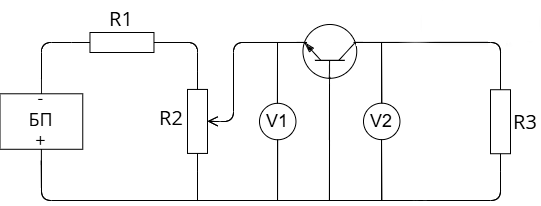
\includegraphics[width=0.8\textwidth]{Схема установки}
\caption{Схема установки}
\label{fig:Схема установки}
\end{figure}
На этой схеме БП – блок питания электрической схемы; R1 – ограничительный
резистор; R2 – потенциометр, с помощью которого можно изменять напряжение $U_{\text{эб}}$; V1 – вольтметр для измерения $U_{\text{эб}}$; R3 – резистор в цепи к-б,по падению напряжения на котором можно измерить ток коллектора $I_{\text{к}}$; V2 – вольтметр для измерения падения напряжения $U_{\text{кб}}$ на R3.
\parСопротивление резистора R3 выбрано достаточно малым (12,0Ом), чтобы
можно было считать цепь коллектора короткозамкнутой.


\begin{figure}[H]
\centering
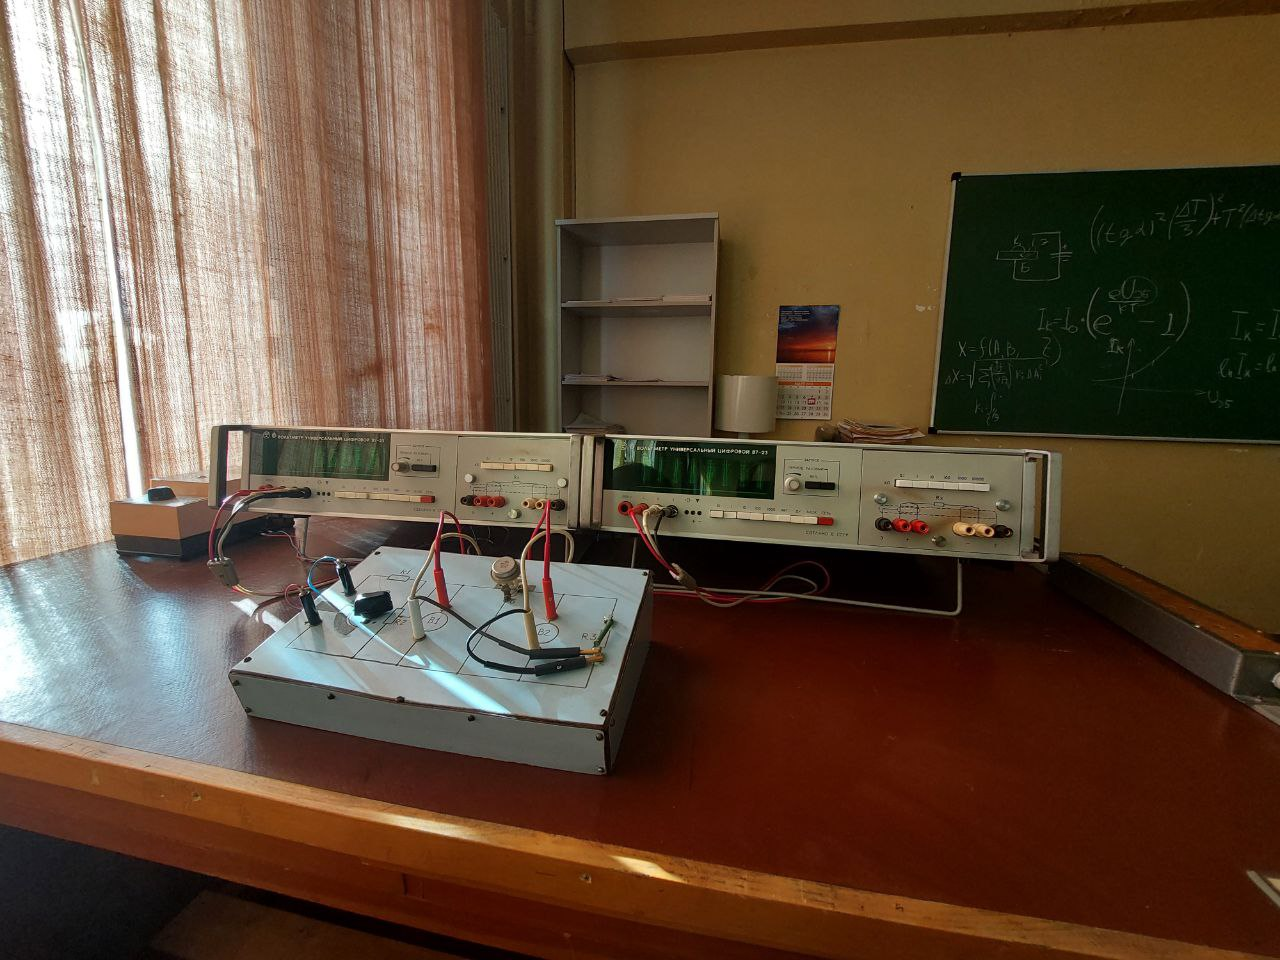
\includegraphics[width=0.8\textwidth]{Установка.jpg}
\caption{Установка}
\label{fig:установка}
\end{figure}

\subsection{Обработка данных и обсуждение результатов}
Вычисление тока коллектора $I_{\text{к}}$ производится по следующей формуле:
\begin{equation}
   I_{\text{к}}=\frac{U_{\text{кб}}}{R3}
   \label{eq:5}
\end{equation}

Разрешение шкалы для вольтметра V1 (для измерений $U_{\text{эб}}$) - два знака после запятой. Разрешение шкалы для вольтметра V2 (для измерений $U_{\text{кб}}$) - четыре знака после запятой. 16 измерений, результаты представлены в таблице \ref{t1}.

\begin{center}
\begin{table}[h!]
\centering
\caption*{Таблица 1. Результаты измерения напряжения и тока}

\label{t1}
\begin{tabular}{|c|c|c|c|c|}
\hline
\begin{minipage}{7mm}
    № п.п. 
\end{minipage}&
\begin{minipage}{3cm}
    \begin{center} $U_{\text{эб}}$ \end{center}
\end{minipage} &
\begin{minipage}{3cm}
    \begin{center} $U_{\text{кб}}$ \end{center}
\end{minipage} &
\begin{minipage}{3cm}
    \begin{center} $I_{\text{к}}=\frac{U_{\text{кб}}}{R3}$ \end{center}
\end{minipage}&
\begin{minipage}{3cm}
   \begin{center} $\ln I_k$ \end{center}
\end{minipage}\\
\hline
{}&В&В&мА&-\\
\hline
1 &  0.30  &  0.0020  &  0.17 & -1.8 \\
2 &  0.31  &  0.0028  & 0.23  & -1.5 \\
3 &  0.32  &  0.0048  &  0.4 & -0.92\\
4 & 0.33  &  0.0112  &  0.93 & -0.073\\
5 & 0.34  &  0.0162  &  1.3 & 0.34\\
6 & 0.35  &  0.0255  &  2.1 & 0.74\\
7 & 0.36  &  0.0362  &  3.0 & 1.1\\
8 & 0.37  &  0.0470  &  3.9 & 1.4\\
9& 0.38  &  0.0745  &   6.2 & 1.8\\
10 &  0.39  &  0.0940  &  7.8 &  2.1\\
11 &  0.40  &  0.1215  &  10 & 2.3\\
12 &  0.41  & 0.1490 &  12 & 2.5\\
13 & 0.42 &  0.1560  &  13 & 2.6\\
14 & 0.43  &  0.1975  &  16 & 2.8\\
15 & 0.44  &  0.2150  & 18  & 2.9\\
16 & 0.45  &  0.2430  &  20 & 3.0\\
\hline
\end{tabular}
\end{table}
\end{center}


Разрешение шкалы для вольтметра V1 (для измерений $U_{\text{эб}}$) - четыре знака после запятой. Разрешение шкалы для вольтметра V2 (для измерений $U_{\text{кб}}$) - четыре знака после запятой. 16 измерений, результаты представлены в таблице ~\ref{tabl:1'}.
\begin{center}
\begin{table}[H]
\centering
\caption*{Таблица 1'. Результаты измерения напряжения и тока}
\label{tabl:1'}
\begin{tabular}{|c|c|c|c|c|}
\hline
\begin{minipage}{7mm}
    № п.п. 
\end{minipage}&
\begin{minipage}{3cm}
   \begin{center} $U_{\text{эб}}$ \end{center}
\end{minipage} &
\begin{minipage}{3cm}
   \begin{center} $U_{\text{кб}}$ \end{center}
\end{minipage} &
\begin{minipage}{3cm}
    \begin{center} $I_{\text{к}}=\frac{U_{\text{кб}}}{R3}$ \end{center}
\end{minipage}&
\begin{minipage}{3cm}
   \begin{center} $\ln I_k$ \end{center}
\end{minipage}\\
\hline
{}&В&В&мА&-\\
\hline
1 &  0.3000  &  0.0016  & 0.13  & -2.0 \\
2 &  0.3100  &  0.0028  & 0.23  & -1.5\\
3 &  0.3200  &  0.0050  & 0.42  & -0.87\\
4 & 0.3300  &  0.0083  & 0.69  & -0.37\\
5 & 0.3400  &  0.0137  &  1.1 & 0.095\\
6 & 0.3500  &  0.0220  &  1.8 & 0.59\\
7 & 0.3600  &  0.0311  &  2.6 & 0.96\\
8 & 0.3700  &  0.0423  &  3.5 & 1.3\\
9& 0.3800  &  0.0600 &  5 &  1.6\\
10 &  0.3900 &  0.0795  &  6.6 & 1.9 \\
11 &  0.4000  &  0.1025  &  8.5 & 2.1\\
12 &  0.4100  & 0.1300 &  11 & 2.4\\
13 & 0.4200 &  0.1543  &  13 & 2.6\\
14 & 0.4300  &  0.1870  &  16 & 2.8\\
15 & 0.4400  &  0.2130  &  18 & 2.9\\
16 & 0.4500  &  0.2363  &  20 & 3.0\\
\hline
\end{tabular}
\end{table}
\end{center}
Методом парных точек найти тангенс угла наклона линейной
зависимости . Процесс вычисления проиллюстрирован таблицами 2 и 2'. В которых $x \rightarrow{} U_{\text{эб}}$, $y\rightarrow{} \ln I_{\text{к}}$.
\begin{center}
\begin{table}[H]
\centering
\caption*{Таблица 2. Метод парных точек}
\label{tabl:2}
\begin{tabular}{|c|c|c|c|c|c|c|c|c|c|}
\hline
\begin{minipage}{7mm}
    № п.п. 
\end{minipage}&
\begin{minipage}{7mm}
   \begin{center} $x_{\text{II}}$ \end{center} 
\end{minipage} &
\begin{minipage}{7mm}
   \begin{center} $x_{\text{I}}$ \end{center} 
\end{minipage} &
\begin{minipage}{14mm}
   \begin{center} $x_{\text{II}}-x_{\text{I}}$ \end{center} 
\end{minipage}&
\begin{minipage}{7mm}
   \begin{center} $y_{\text{II}}$ \end{center} 
\end{minipage}&
\begin{minipage}{7mm}
   \begin{center} $y_{\text{I}}$ \end{center} 
\end{minipage}&
\begin{minipage}{14mm}
   \begin{center} $y_{\text{II}}-y_{\text{I}}$ \end{center} 
\end{minipage}&
\begin{minipage}{25mm}
   \begin{center} $a_{\text{i}}=\frac{y_{\text{II}}-y_{\text{I}}}{x_{\text{II}}-x_{\text{I}}}$ \end{center} 
\end{minipage}&
\begin{minipage}{21mm}
     \begin{center} $(a_{\text{i}}-\overline{a})$ \end{center}
\end{minipage}&
\begin{minipage}{21mm}
     \begin{center} $(a_{\text{i}}-\overline{a})^2$ \end{center}
\end{minipage}\\
\hline
1 &  0.38  &  0.30  & 0.080 & 1.8& -1.8&3.6 & 45.0 &13 & 169.0\\
2 &  0.39  &  0.31  &  0.080 & 2.1& -1.5&3.6 &45.0 &13 &169.0\\
3 &  0.40  &  0.32  & 0.080  & 2.3& -0.92&3.2 &40.0 &7.5 &60.84\\
4 & 0.41  &  0.33 &  0.080 & 2.5& -0.073&2.6  &32.5 &0 & 0\\
5 & 0.42  &  0.34  &  0.080 &  2.6&0.34 &2.3 &28.8 &-4.1 & 16.81 \\
6 & 0.43  &  0.35  &  0.080 & 2.8&0.74 &2.1 &26.3 &-6.7 & 44.89\\
7 & 0.44  &  0.36  &  0.080 & 2.9&1.1 &1.8 &22.5 &-9.9 & 98.01 \\
8 & 0.45  &  0.37  &  0.080 & 3.0& 1.4 &1.6 &20.0 &-12 & 144 \\
 &   &    &   & &  & & $\Sigma=260.1$& & $\Sigma=715.38$ \\
\hline
\end{tabular}
\end{table}
\end{center}
\parБыли высчитаны следующие величины для значений таблицы 2.
\begin{equation}
    tg{\alpha}=\overline{a}=32.5
\end{equation}
Погрешность $tg{\alpha}$ вычислена по формуле:
\begin{equation}
    \Delta\overline{a}=t_{\alpha,n}\cdot\frac{\sqrt{\frac{\Sigma(a_i-\overline{a})^2}{{n-1}}}}{\sqrt{n}}=8.5
\end{equation}
где $t_{\alpha,n}=2.4$.
\parОтношение $\frac{e}{k}$=9624.88К/В, высчитано по формуле~\ref{eq:eq4}.Погрешность отношения высчитывается как погрешность косвенных измерений по формуле:
\begin{equation}
    \Delta\frac{e}{k}=\sqrt{\overline{a}^2(\frac{\Delta T}{3})^2+T^2(\Delta\overline{a})^2}=2546.9 \text{К/В}
\end{equation}
\begin{center}
\begin{table}[H]
\centering
\caption*{Таблица 2'. Метод парных точек}
\label{tabl:2}
\begin{tabular}{|c|c|c|c|c|c|c|c|c|c|}
\hline
\begin{minipage}{7mm}
    № п.п. 
\end{minipage}&
\begin{minipage}{7mm}
   \begin{center} $x_{\text{II}}$ \end{center} 
\end{minipage} &
\begin{minipage}{7mm}
   \begin{center} $x_{\text{I}}$ \end{center} 
\end{minipage} &
\begin{minipage}{14mm}
   \begin{center} $x_{\text{II}}-x_{\text{I}}$ \end{center} 
\end{minipage}&
\begin{minipage}{7mm}
   \begin{center} $y_{\text{II}}$ \end{center} 
\end{minipage}&
\begin{minipage}{7mm}
   \begin{center} $y_{\text{I}}$ \end{center} 
\end{minipage}&
\begin{minipage}{14mm}
   \begin{center} $y_{\text{II}}-y_{\text{I}}$ \end{center} 
\end{minipage}&
\begin{minipage}{23mm}
   \begin{center} $a_{\text{i}}=\frac{y_{\text{II}}-y_{\text{I}}}{x_{\text{II}}-x_{\text{I}}}$ \end{center} 
\end{minipage}&
\begin{minipage}{18mm}
     \begin{center} $(a_{\text{i}}-\overline{a})$ \end{center}
\end{minipage}&
\begin{minipage}{21mm}
     \begin{center} $(a_{\text{i}}-\overline{a})^2$ \end{center}
\end{minipage}\\
\hline
1 &  0.3800  &  0.3000  & 0.0800 & 1.6& -2.0&3.600 & 45.000 &12.04 & 144.962\\
2 &  0.3900  &  0.3100  &  0.0800 & 1.9& -1.5&3.400 &45.000 &9.539 &90.9925\\
3 &  0.4000  &  0.3200  & 0.0800  & 2.1& -0.87&2.200 &40.200 &4.164 &17.3389\\
4 & 0.4100  &  0.3300 &  0.0800 & 2.4& -0.37&2.600  &32.200 &1.664 &2.76890\\
5 & 0.4200  &  0.3400  &  0.0800 &  2.6&0.095 &2.260 &28.300 &-1.648 &2.71590  \\
6 & 0.4300  &  0.3500  &  0.0800 & 2.8&0.59 &2.100 &25.700 &-5.336 &28.4729 \\
7 & 0.4400  &  0.3600  &  0.0800 & 2.9&0.96 &1.800 &22.500 &-8.711 & 75.8815 \\
8 & 0.4500  &  0.3700  &  0.0800 & 3.0& 1.3 &1.600 &20.000 &-11.71 &137.12400  \\
 &   &    &   & &  & & $\Sigma=263.688$& & $\Sigma=500.25600$ \\

\hline
\end{tabular}
\end{table}
\end{center}
\parБыли высчитаны следующие величины для значений таблицы 2.
\begin{equation}
    tg{\alpha}=\overline{a}=32.961
\end{equation}
Погрешность$tg{\alpha}$ вычислена по формуле:
\begin{equation}
    \Delta\overline{a}=t_{\alpha,n}\cdot\frac{\sqrt{\frac{\Sigma(a_i-\overline{a})^2}{{n-1}}}}{\sqrt{n}}=7.173
\end{equation}
где $t_{\alpha,n}=2.4$.
\parОтношение $\frac{e}{k}$=9761.4К/В, высчитано по формуле~\ref{eq:eq4}.Погрешность отношения высчитывается как погрешность косвенных измерений по формуле:
\begin{equation}
    \Delta\frac{e}{k}=\sqrt{\overline{a}^2(\frac{\Delta T}{3})^2+T^2(\Delta\overline{a})^2}=2124.29 \text{К/В}
\end{equation}



\subsubsection{Графики}
Вычислим $\ln I_0$ по формуле:
\begin{equation}
    \ln I_0=\overline{\ln I_k}-\frac{e}{kT}\overline{U_{\text{эб}}}
\end{equation}
Для таблицы 1 были получены следующие значения $\ln I_0$=0.1, $I_0$=1.1мА.
Для таблицы 1' были получены следующие значения $\ln I_0$=0.1, $I_0$=1.1мА.

\section{Выводы}



\begin{thebibliography}{9}

%ссылка на репозиторий с исходныим кодом отчета и всех расчетных программ 
\bibitem{repo}
\url{https://github.com/st117207/Workshop2}  (дата обращения: 29.03.2024) 


\end{thebibliography}

